\clearpage
\newpage
\subsubsection{Estensione B: Ripristino di un Annuncio Precedente}
Se l’utente sceglie di \textbf{ripristinare l’annuncio precedente}, il sistema avvia un processo di caricamento per fornire un feedback visivo sulla ripresa dei dati. Sebbene i dati siano salvati localmente e il recupero sia immediato, un \textbf{indicatore di caricamento fittizio} viene mostrato per alcuni secondi prima di caricare la schermata.

Questa soluzione è basata sul principio della \textbf{coerenza con le aspettative dell’utente} \cite{shneiderman2004}. In un contesto digitale, un ripristino istantaneo potrebbe apparire innaturale e creare confusione. L’indicatore di caricamento:
\begin{itemize}
    \item Rafforza la percezione di un processo in corso, migliorando la trasparenza dell’operazione.
    \item Evita che l’utente si domandi se il recupero sia realmente avvenuto o se ci siano stati problemi tecnici.
    \item Contribuisce a una transizione più fluida tra stati dell’interfaccia.
\end{itemize}

Una volta completato il caricamento, il sistema presenta l’interfaccia con i dati precedentemente salvati, consentendo all’utente di riprendere il processo da dove era stato interrotto.


\begin{figure}[ht]
    \centering
    \begin{tikzpicture}[node distance=1.5cm and 1cm, auto]
        % Nodo per immagine 1 con didascalia sotto
        \node (img1) {
            \begin{tabular}{c}
                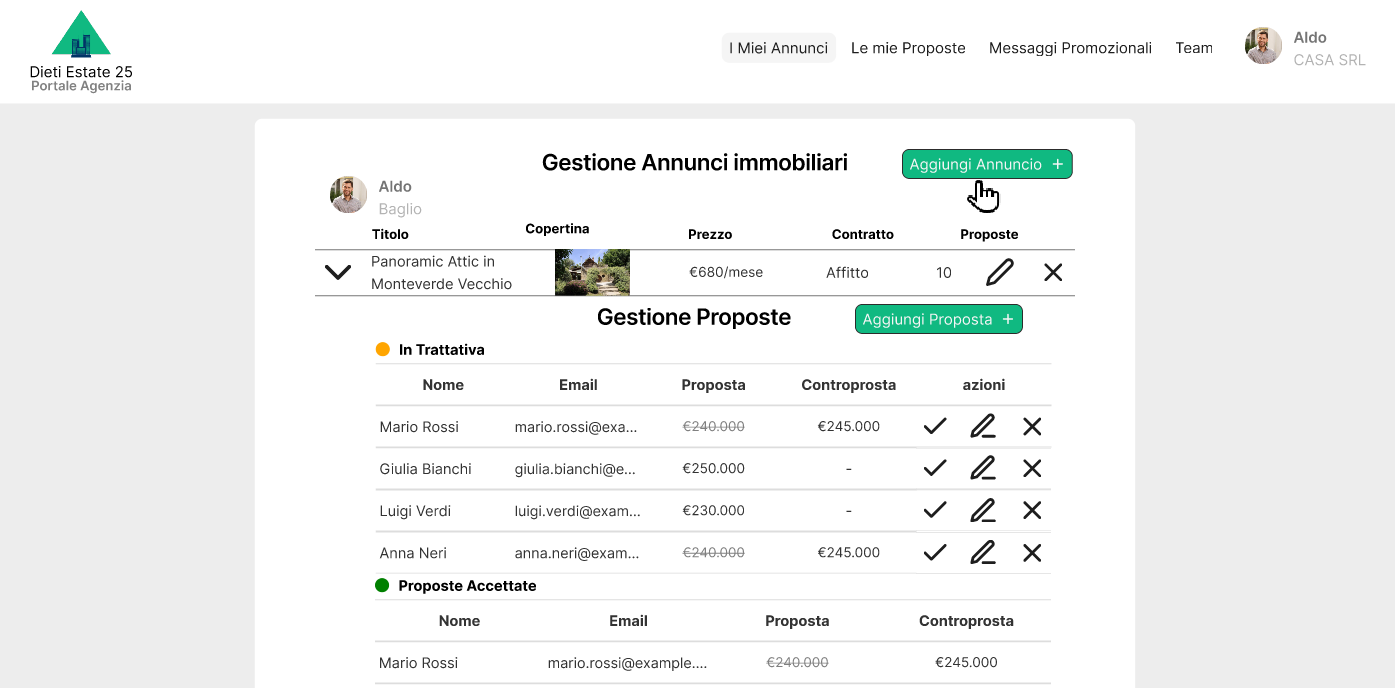
\includegraphics[width=0.7\textwidth]{Immagini/Mockup/aggiungi annuncio/estensione B/step1.png} \\
                click nuovo annuncio
            \end{tabular}
        };
        
        % Nodo per immagine 2 con didascalia sotto, posizionato a destra di img1
        \node (img2) [below=of img1] {
            \begin{tabular}{c}
                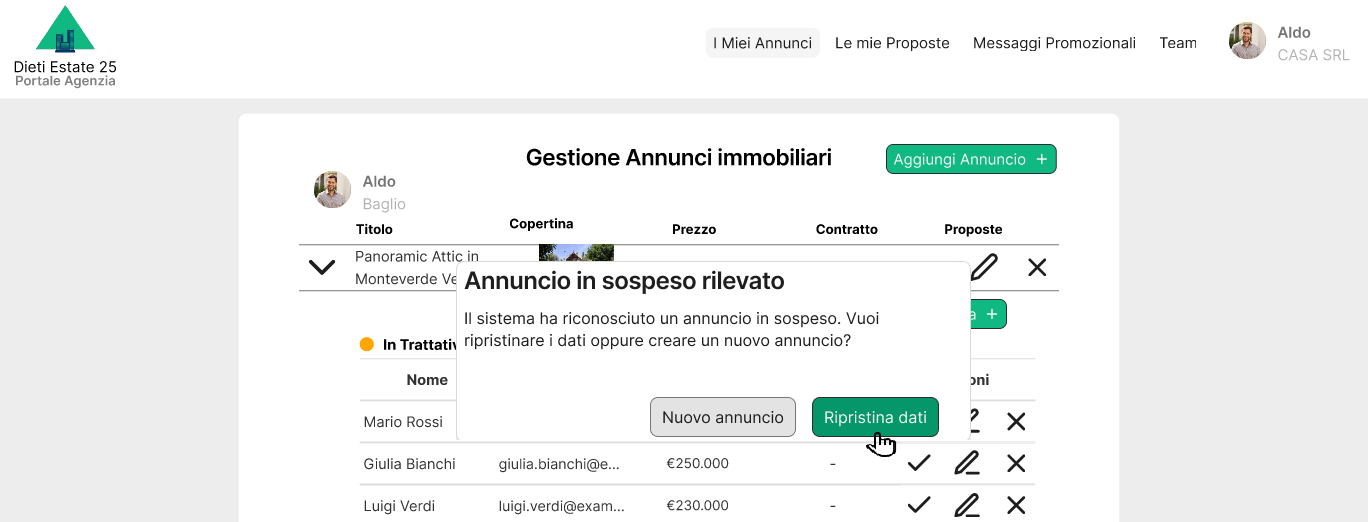
\includegraphics[width=0.7\textwidth]{Immagini/Mockup/aggiungi annuncio/estensione B/step2.png} \\
                Cockburn: extension B.2/B.3/B.4
            \end{tabular}
        };
        
        % Nodo per immagine 3 con didascalia sotto, posizionato sotto img2
        \node (img3) [below=of img2] {
            \begin{tabular}{c}
                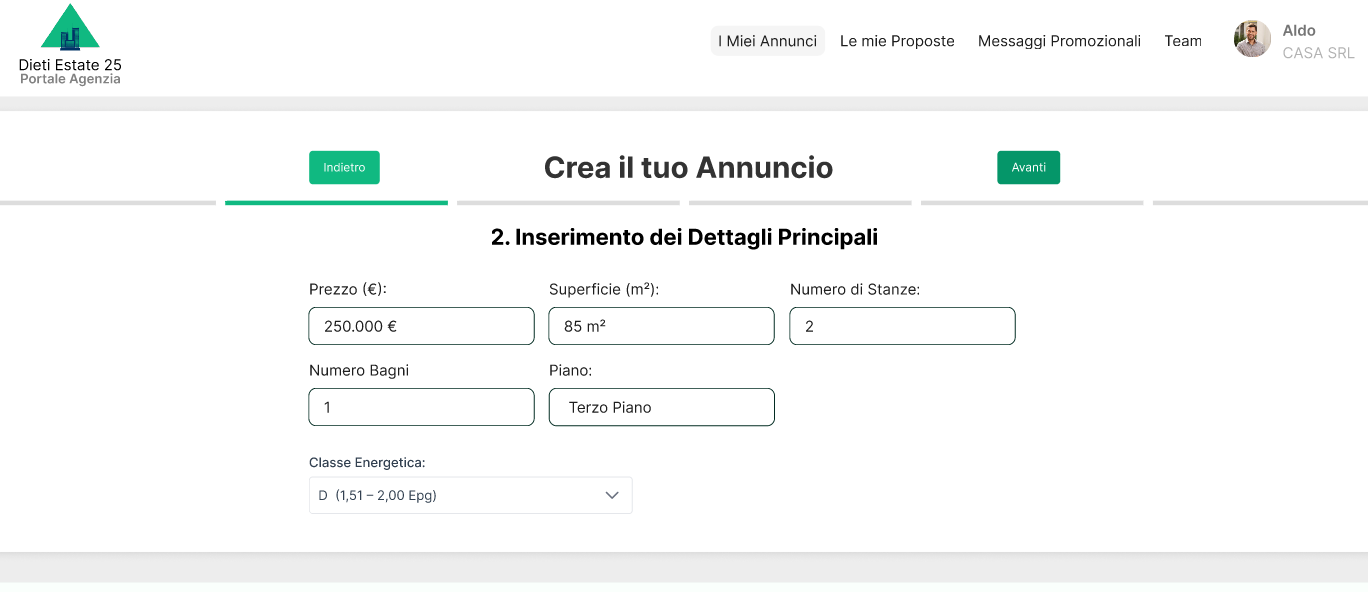
\includegraphics[width=0.7\textwidth]{Immagini/Mockup/aggiungi annuncio/estensione B/step3.png} \\
                Cockburn: extension B.5
            \end{tabular}
        };
        
        % Disegna le frecce
        \draw[->, thick] (img1) -- (img2);
        \draw[->, thick] (img2) -- (img3);
      
    \end{tikzpicture}
    \caption{Mockup: estensione B della tabella di Cockburn del caso d'uso nuovo annuncio}
    \label{fig:tikz_flow}
\end{figure}

\newpage

